\chapter{System Design}

%Replace \lipsum with text.
% You may have as many sections as you please. This is just for reference.

\section{High Level Design}
%\lipsum[2]
% You may add figures in the following manner.

\begin{figure}[here]
\begin{center}	
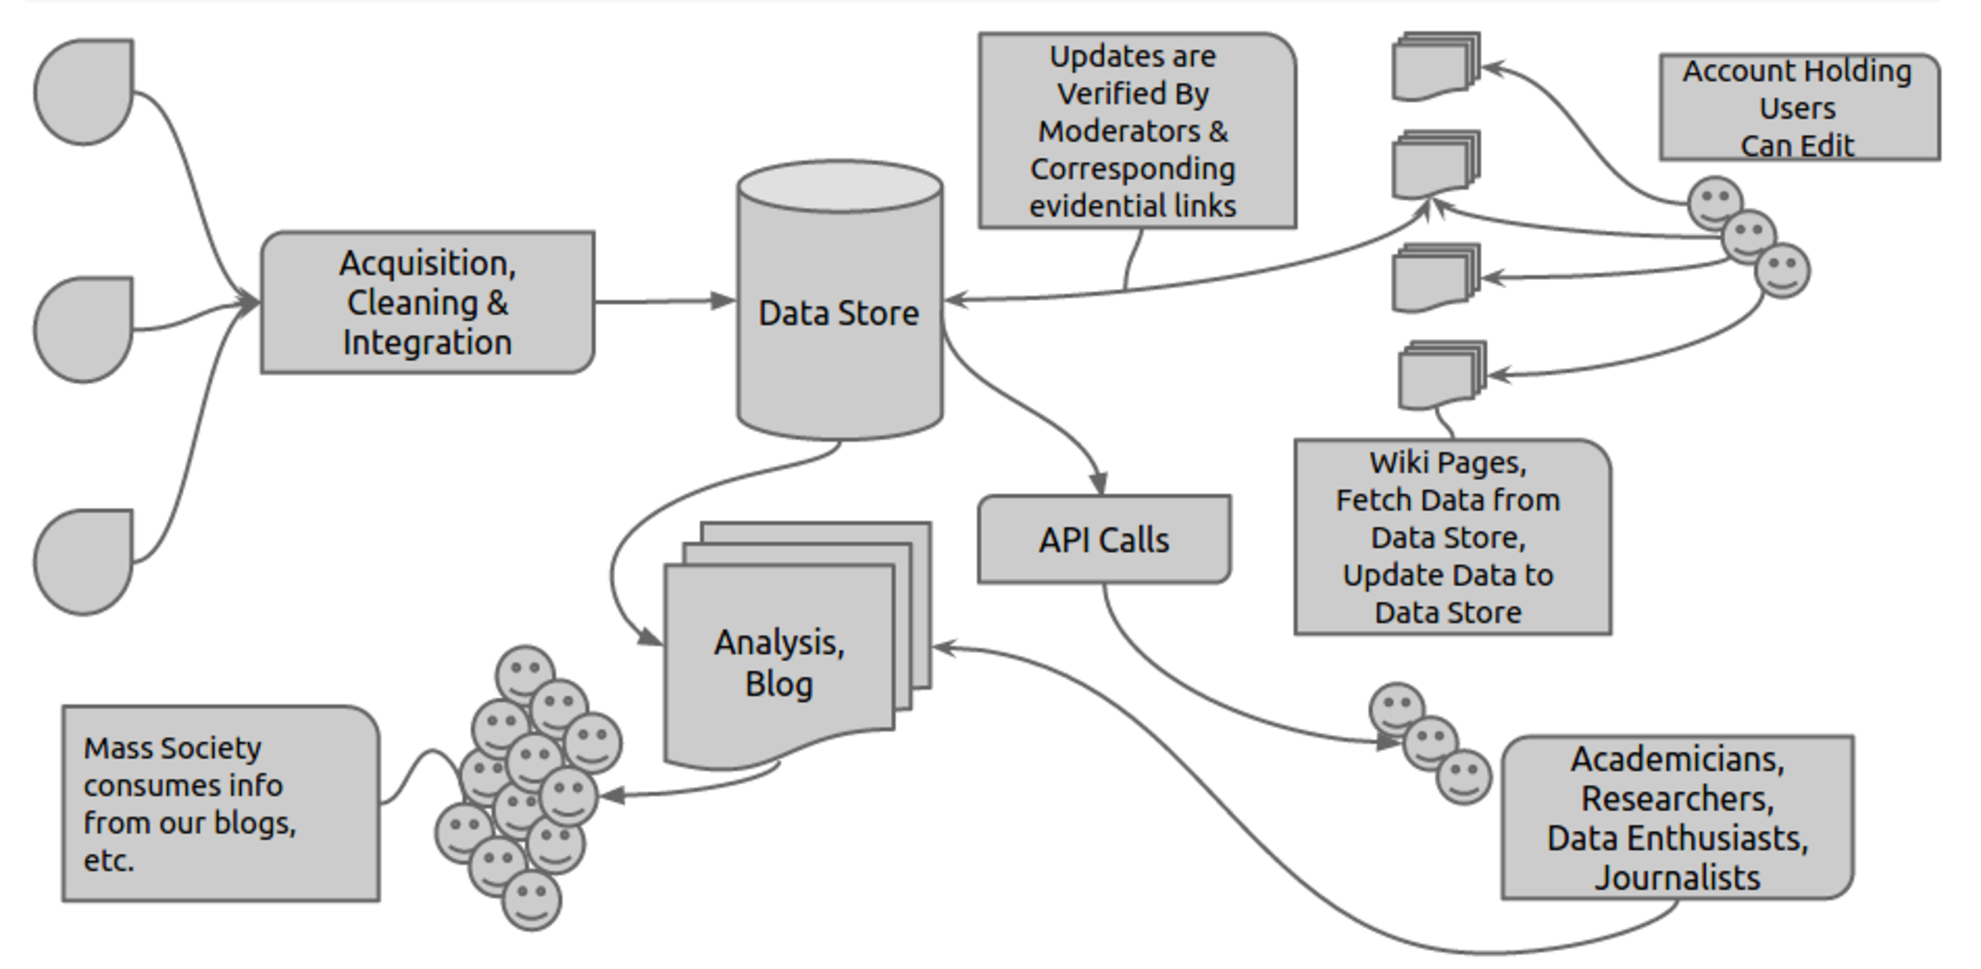
\includegraphics[scale=0.4]{big_pic} 
\caption{Big Picture}
\label{fig:big_pic}
\end{center}
\end{figure}

Above is the generic high level diagram of the entire system as we deduced from our study of the websites above.
We have assumed three main types of users of here:
\begin{enumerate}
\item\textbf{General public} - Use the system for information and news. May also contribute towards data entry.
\item\textbf{Researchers \& Academicians} - Use the site for using social network studies.
\item\textbf{Journalists (Media persons)} - Use the data to frame their news stories.
\end{enumerate}


And keeping these in mind, the system accounts for following functions:
\begin{itemize}
\item\textbf{Data acquisition} - As getting structured data is often difficult system should have a mechanism to automate collection of data from various sources over internet.
\item\textbf{Data Store}  - There should be a central repository for whatever data collected. This repo will store the data in structured form. Care should be taken to keep its integrity, durability and non-redundancy.
\item\textbf{Data Verification} - As the data is sensitive and important, provisions for verification for the input data has to be taken care of. This involves manual labor and system should incorporate this in the entire process.
\item\textbf{Data Visualization} - A portal for the public display of data (in tables, visualizations etc.).
\item\textbf{APIs} - To provide our data for use with other applications.
\end{itemize}

\section{Technical design}
%\lipsum[3]
Accordingly we have incorporated the functionalities in the following way:\\

\begin{figure}[here]
\begin{center}	
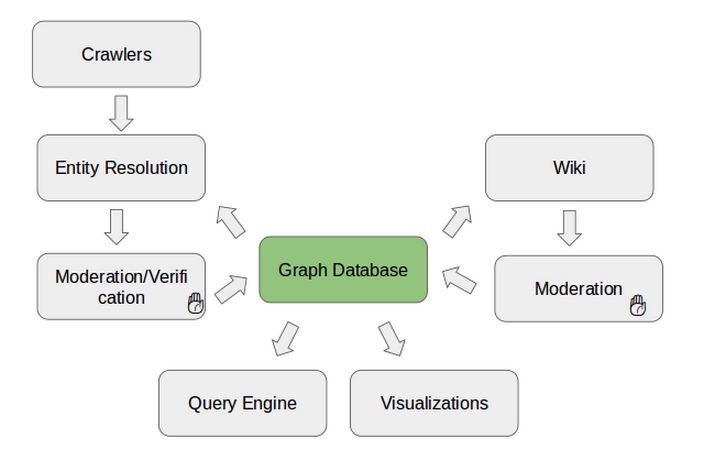
\includegraphics[scale=0.4]{tech_pic} 
\caption{Proposed System}
\label{fig:tech_pic}
\end{center}
\end{figure}

Components include:
\begin{itemize}
\item\textbf{Crawlers-Cleaner-Resolver} - As a part of the data acquisition module, the crawler crawls specific websites and scrapes data in format specified in a static file. Cleaner and resolver works on the scraped data. The cleaner makes the data more structured by keeping all data in specific format, discarding missing values etc. The resolver acts on the data to remove all duplicate entries (and merge similar entries) so to keep the data non redundant as possible.
\item\textbf{Verifier}- The data coming from the crawler after resolution is verified by human moderator. Any to-be-updated information is first human moderated. Any new data is then fed to the graph database.
\item\textbf{Graph database} - Acts as the data store for the system storing structured data with nodes as entities and edges as relationships.
\item\textbf{Web portal(Query Engine, Visualization, Wiki)} - This is the final product that is directly visible to the users. All visualizations (graphical, tabular) are done here. It also has an wiki interface for an end user to add more entities/relations to the graph database. The portal also includes a query/search engine to show results as per specific user queries.
\item\textbf{API} - Registered users can use this to read in data from the datastore in their application.
\end{itemize} 

%\section{SECTION NAME}
%\lipsum[2]
